\section{CONSGD}

\subsection{Algorithm}
\begin{frame}
    \frametitle{Algorithm}
	\begin{itemize}
		\item CONSGD uses a constant global learning rate and multiplies it to each local update. 
		\item $w\gets w+\lambda u_{c}^{m} $, $\lambda \in (0,1)$
	\end{itemize}
\end{frame}

\subsection{Intuition}
\begin{frame}
    \frametitle{Intuition}
	\begin{figure}
		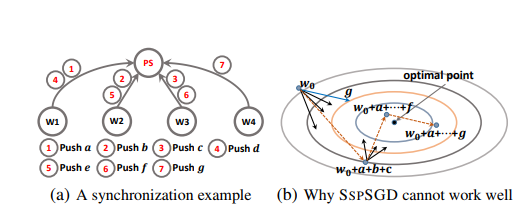
\includegraphics[scale=0.5]{figure/intuition.png}
	\end{figure} 
\end{frame}

\begin{frame}
	\frametitle{Why CONSGD works better?}
	\begin{figure}
		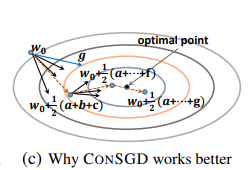
\includegraphics[scale=0.8]{figure/consgdwork.png}
	\end{figure}
\end{frame}



\subsection{Choose $\lambda$}
\begin{frame}
    \frametitle{Choose $\lambda$}
	\begin{itemize}
		\item $w_{c+1}=\frac{1}{M}\sum_{i=1}^{M}(w_{c}+u_{c}^{i})=w_{c}+\frac{1}{M}\sum_{i=1}^{M}u_{c}^{i}$
		\item $\lambda = \frac{1}{M}$ is a good choice. 
	\end{itemize} 
\end{frame}

\subsection{Limitation}
\begin{frame}
    \frametitle{Limitation}
	\begin{figure}
		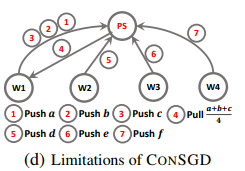
\includegraphics[scale=0.8]{figure/consgdlimit.png}
	\end{figure}
\end{frame}


